\documentclass{ibetest}
\begin{document}
\maketest{End-of-Unit Test --- Thermo-S1 Part 1}
         {Description of a system in thermodynamics \,$\cdot$\, sections 1.A to 3.C}
         {45 minutes}{50}

% ---------------------------------------------------------------------------
\exercise[1.A $\cdot$ 1.B $\cdot$ 2.A]{Unit conversions}{3 marks}
Give each result exactly, without rounding.\\
(a) $V = \qty{350}{mL}$ in $\mathrm{m^3}$. \quad
(b) $\theta = \qty{-40}{\degreeCelsius}$ in kelvins. \quad
(c) $\chi_T = \qty{5.0e-10}{\per\pascal}$ in $\mathrm{bar^{-1}}$.
\answer{1,1,1}{3.4cm}{%
  (a) $V = 350\times10^{-3}\ \mathrm L = 0.350\times10^{-3}\ \mathrm{m^3}$ \qquad
      $\boxed{V = 3.50\times10^{-4}\ \mathrm{m^3}}$\\[3pt]
  (b) $T = \theta + 273.15 = -40 + 273.15$ \qquad $\boxed{T = 233.15\ \mathrm K}$\\[3pt]
  (c) $1\ \mathrm{Pa^{-1}} = 10^{5}\ \mathrm{bar^{-1}}$ \qquad
      $\boxed{\chi_T = 5.0\times10^{-5}\ \mathrm{bar^{-1}}}$}
\begin{scheme}
\pt{1}{1 pt}{$3.50\times10^{-4}\ \mathrm{m^3}$.}
\pt{2}{1 pt}{$233.15$~K (capital K, no degree sign).}
\pt{3}{1 pt}{$5.0\times10^{-5}\ \mathrm{bar^{-1}}$.}
\end{scheme}

% ---------------------------------------------------------------------------
\exercise[1.A]{Extensive and intensive quantities --- definitions}{5 marks}
Define an extensive quantity and an intensive quantity, giving two examples of each. Show
that the molar volume $V_m = V/n$ is intensive.
\answer{2,2,1}{5.6cm}{%
  An \textbf{extensive} quantity is proportional to the size (amount of matter) of the system:
  if the system is doubled, it doubles, e.g.\ $V(2n) = 2V(n)$. Examples: mass $m$, volume
  $V$, amount of substance $n$, energy $E$.\\[4pt]
  An \textbf{intensive} quantity does not depend on the size of the system: it keeps the same
  value when the system is doubled. Examples: pressure $p$, temperature $T$, mass density
  $\rho$.\\[4pt]
  $V_m = V/n$: doubling the system doubles both $V$ and $n$, so their ratio is unchanged. The
  quotient of two extensive quantities is intensive.}
\begin{scheme}
\pt{1}{2 pts}{Extensive: proportional to the size / doubles with the system (1~pt); two
  examples (1~pt).}
\pt{2}{2 pts}{Intensive: independent of the size (1~pt); two examples (1~pt).}
\pt{3}{1 pt}{$V_m$ intensive, justified.}
\end{scheme}

% ---------------------------------------------------------------------------
\exercise[1.A $\cdot$ 1.B]{Systems and equilibrium}{3 marks}
\question{A weather balloon (sealed, flexible envelope) is:}
\opttwo{0}{open}{1}{closed but not isolated}{0}{isolated}{0}{neither closed nor open}
\why{no matter crosses the sealed envelope (closed), but heat and work are exchanged (the
  envelope is flexible and not insulating).}
\question{A gas in an insulating cylinder closed by a rigid lid is:}
\opttwo{1}{isolated}{0}{open}{0}{closed but not isolated}{0}{necessarily at 0~K}
\why{sealed (no matter), rigid (no work) and insulating (no heat): Fig.~2 of the notes.}
\question{Thermodynamic equilibrium requires:}
\optlist{0}{only a steady state;}
        {0}{only homogeneity;}
        {1}{both: $p$ and $T$ uniform in space and constant in time, and equal to those of the
            surroundings;}
        {0}{only thermal equilibrium.}
\why{``the pressure and the temperature [must] depend neither on space (homogeneity) nor on
  time (steady state)''.}

% ---------------------------------------------------------------------------
\exercise[1.C $\cdot$ 2.B]{State diagrams and coefficients}{4 marks}
\question{The slope of an isotherm drawn as $V$ versus $p$ is:}
\opts{1}{$\left(\frac{\partial V}{\partial p}\right)_T$}{0}{$\left(\frac{\partial V}{\partial T}\right)_p$}
     {0}{$\left(\frac{\partial p}{\partial T}\right)_V$}{0}{$V/p$}
\why{on an isotherm $T$ is fixed, and the slope of $V(p)$ is the partial derivative at fixed
  $T$.}
\question{For a gas, the sign of $\left(\frac{\partial V}{\partial T}\right)_p$ is:}
\opts{1}{positive}{0}{negative}{0}{zero}{0}{undetermined}
\why{at fixed pressure a heated gas expands (Fig.~7).}
\question{The piezothermic coefficient is defined by:}
\opts{1}{$\frac1p\left(\frac{\partial p}{\partial T}\right)_V$}{0}{$\frac1V\left(\frac{\partial V}{\partial T}\right)_p$}
     {0}{$-\frac1V\left(\frac{\partial V}{\partial p}\right)_T$}{0}{$\frac1T\left(\frac{\partial T}{\partial p}\right)_V$}
\why{Tab.~3: $\beta$ describes $p$ at fixed $V$. The others are $\alpha$ and $\chi_T$.}
\question{The SI unit of $\chi_T$ is:}
\opts{1}{$\mathrm{Pa^{-1}}$}{0}{$\mathrm{K^{-1}}$}{0}{$\mathrm{Pa}$}{0}{no unit}
\why{$\chi_T = -\frac1V\left(\frac{\partial V}{\partial p}\right)_T$ is the inverse of a
  pressure.}

% ---------------------------------------------------------------------------
\exercise[2.A $\cdot$ 2.C]{A sealed container full of water}{6 marks}
A steel container, assumed rigid, is completely filled with liquid water and sealed. The
coefficients of water are given below.
(a) Write $\dd V$ in terms of $\alpha$, $\chi_T$, $\dd T$ and $\dd p$.
(b) Deduce $\left(\frac{\partial p}{\partial T}\right)_V$ and compute it.
(c) Estimate the pressure rise $\Delta p$ when the water is heated by $\Delta T$.
(d) Compare with an ideal gas at $p = \qty{1.0e5}{Pa}$ and $T = \qty{300}{K}$, and conclude.
\data{$\alpha = \qty{2.0e-4}{\per\kelvin}$ \hspace{12mm} $\chi_T = \qty{5.0e-10}{\per\pascal}$
      \hspace{12mm} $\Delta T = \qty{5.0}{K}$}
\answer{1,1,1,1,1,1}{7.8cm}{%
  (a) $\dd V = \left(\dfrac{\partial V}{\partial T}\right)_{\!p}\dd T
     + \left(\dfrac{\partial V}{\partial p}\right)_{\!T}\dd p$ \qquad so \qquad
     $\boxed{\dd V = \alpha V\,\dd T - \chi_TV\,\dd p}$\\[4pt]
  (b) The container is rigid, so $\dd V = 0$:\quad
     $\boxed{\left(\dfrac{\partial p}{\partial T}\right)_{\!V} = \dfrac{\alpha}{\chi_T}}
     = \dfrac{2.0\times10^{-4}}{5.0\times10^{-10}} = 4.0\times10^{5}\ \mathrm{Pa\,K^{-1}}$
     \ (4~bar per kelvin)\\[4pt]
  (c) $\Delta p\approx\dfrac{\alpha}{\chi_T}\Delta T = 4.0\times10^{5}\times5.0$ \qquad
     $\boxed{\Delta p\approx2.0\times10^{6}\ \mathrm{Pa} = 20\ \mathrm{bar}}$\\[4pt]
  (d) Ideal gas at fixed $V$: $\left(\dfrac{\partial p}{\partial T}\right)_{\!V} = \dfrac pT
     = \dfrac{1.0\times10^{5}}{300}\approx3.3\times10^{2}\ \mathrm{Pa\,K^{-1}}$, about
     $10^{3}$ times smaller.\\[2pt]
  A liquid is almost incompressible, so even gentle heating in a closed full container
  builds up an enormous pressure: the container bursts. This is why heating circuits have
  expansion tanks.}
\begin{scheme}
\pt{1}{1 pt}{$\dd V = \alpha V\dd T - \chi_TV\dd p$.}
\pt{2}{1 pt}{$\dd V = 0$, so $\left(\partial p/\partial T\right)_V = \alpha/\chi_T$.}
\pt{3}{1 pt}{$4.0\times10^{5}\ \mathrm{Pa\,K^{-1}}$.}
\pt{4}{1 pt}{$\Delta p\approx2.0\times10^{6}\ \mathrm{Pa}$ (20~bar).}
\pt{5}{1 pt}{Ideal gas: $p/T\approx3.3\times10^{2}\ \mathrm{Pa\,K^{-1}}$.}
\pt{6}{1 pt}{Conclusion: ratio about $10^3$, danger of heating a full sealed container.}
\end{scheme}

% ---------------------------------------------------------------------------
\exercise[2.C $\cdot$ 3.A]{Thermoelastic coefficients of the ideal gas}{4 marks}
Starting from $pV = nRT$, compute $\alpha$, $\chi_T$ and $\beta$ for an ideal gas, and check
that $\beta = \alpha/(p\chi_T)$.
\answer{1,1,1,1}{5.0cm}{%
  $V = \dfrac{nRT}{p}$: \quad $\alpha = \dfrac1V\dfrac{nR}{p}$, so $\boxed{\alpha = \dfrac1T}$
  \qquad $\chi_T = -\dfrac1V\left(-\dfrac{nRT}{p^2}\right)$, so $\boxed{\chi_T = \dfrac1p}$\\[5pt]
  $p = \dfrac{nRT}{V}$: \quad $\beta = \dfrac1p\,\dfrac{nR}{V}$, so $\boxed{\beta = \dfrac1T}$\\[5pt]
  Check: $\dfrac{\alpha}{p\chi_T} = \dfrac{1/T}{p\cdot1/p} = \dfrac1T = \beta$. \checkmark}
\begin{scheme}
\pt{1}{1 pt}{$\alpha = 1/T$.}
\pt{2}{1 pt}{$\chi_T = 1/p$.}
\pt{3}{1 pt}{$\beta = 1/T$.}
\pt{4}{1 pt}{Relation checked.}
\end{scheme}

% ---------------------------------------------------------------------------
\exercise[3.A]{Historical laws}{5 marks}
(a) An aerosol can (rigid) contains a gas at $p_1$ and $\theta_1$. It is left in the sun and
reaches $\theta_2$. Which law applies? Compute the final pressure $p_2$.
(b) The bubble of a Cartesian diver, of volume $V$ at pressure $p$, is compressed at constant
temperature to the pressure $p'$. Compute its new volume $V'$.
\data{(a) \ $p_1 = \qty{3.0}{bar}$ \hspace{10mm} $\theta_1 = \qty{27}{\degreeCelsius}$
      \hspace{10mm} $\theta_2 = \qty{127}{\degreeCelsius}$\\[2pt]
      (b) \ $V = \qty{1.0}{\centi\metre\cubed}$ \hspace{10mm} $p = \qty{1.0}{bar}$ \hspace{10mm}
      $p' = \qty{1.25}{bar}$}
\answer{1,1,1,1,1}{5.8cm}{%
  (a) $n$ and $V$ are fixed: \textbf{Gay-Lussac's law}, $p/T = $ const., with
  $T_1 = 300\ \mathrm K$ and $T_2 = 400\ \mathrm K$:\\[3pt]
  \hspace*{5mm}$p_2 = p_1\dfrac{T_2}{T_1} = 3.0\times\dfrac{400}{300}\ \mathrm{bar}$ \qquad
  $\boxed{p_2 = 4.0\ \mathrm{bar}}$\\[5pt]
  (b) $n$ and $T$ are fixed: \textbf{Boyle--Mariotte}, $pV = p'V'$:\qquad
  $V' = \dfrac{pV}{p'} = \dfrac{1.0\times1.0}{1.25}\ \mathrm{cm^3}$ \qquad
  $\boxed{V' = 0.80\ \mathrm{cm^3}}$}
\begin{scheme}
\pt{1}{1 pt}{Gay-Lussac identified (fixed $n$ and $V$).}
\pt{2}{1 pt}{Temperatures in kelvins: $300$~K and $400$~K.}
\pt{3}{1 pt}{$p_2 = 4.0$~bar.}
\pt{4}{1 pt}{$V' = pV/p'$ (Boyle--Mariotte).}
\pt{5}{1 pt}{$V' = 0.80\ \mathrm{cm^3}$.}
\end{scheme}

% ---------------------------------------------------------------------------
\exercise[1.B $\cdot$ 3.B]{A piston under a weight}{7 marks}
\noindent\begin{minipage}[c]{0.6\textwidth}
A vertical cylinder of cross-section $S$ is closed by a frictionless piston of mass $M$. The
gas below it, treated as an ideal gas, fills a height $h_1$ at temperature $T_1$. Outside, the
pressure is $p_0$.
(a) Find the pressure $p$ of the gas.
(b) Find the amount of gas $n$.
(c) The gas is heated slowly to $T_2$, the piston remaining free. Find the new height $h_2$
and the displacement of the piston.
\end{minipage}\hfill
\begin{minipage}[c]{0.36\textwidth}\centering
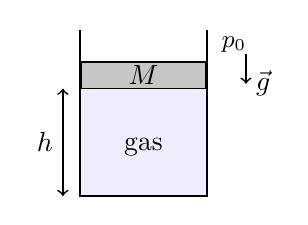
\begin{tikzpicture}[scale=0.62, line width=0.6pt]
  \fill[blue!7] (0,0) rectangle (2.6,2.2);
  \draw (0,3.4) -- (0,0) -- (2.6,0) -- (2.6,3.4);
  \node at (1.3,1.0) {gas};
  \draw[fill=gray!45] (0.03,2.2) rectangle (2.57,2.75); \node at (1.3,2.47) {$M$};
  \draw[<->] (-0.35,0) -- (-0.35,2.2) node[midway, left] {$h$};
  \node[right, font=\small] at (2.7,3.1) {$p_0$};
  \draw[->] (3.4,2.9) -- (3.4,2.3) node[right] {$\vec g$};
\end{tikzpicture}
\end{minipage}
\data{$S = \qty{100}{\centi\metre\squared}$ \hspace{6mm} $M = \qty{20}{kg}$ \hspace{6mm}
      $g = \qty{10}{\metre\per\second\squared}$ \hspace{6mm} $p_0 = \qty{1.0e5}{Pa}$\\[2pt]
      $h_1 = \qty{25}{cm}$ \hspace{6mm} $T_1 = \qty{300}{K}$ \hspace{6mm} $T_2 = \qty{360}{K}$
      \hspace{6mm} $RT_1\approx\qty{2.5e3}{\joule\per\mole}$}
\answer{2,1,1,1,2}{7.6cm}{%
  (a) Equilibrium of the piston: $pS = p_0S + Mg$, so $\boxed{p = p_0 + \dfrac{Mg}{S}}$, with
  $S = 1.0\times10^{-2}\ \mathrm{m^2}$:\\[3pt]
  \hspace*{5mm}$\dfrac{Mg}{S} = \dfrac{20\times10}{1.0\times10^{-2}} = 2.0\times10^{4}\ \mathrm{Pa}$
  \qquad $\boxed{p = 1.2\times10^{5}\ \mathrm{Pa}}$\\[4pt]
  (b) $V_1 = Sh_1 = 1.0\times10^{-2}\times0.25 = 2.5\times10^{-3}\ \mathrm{m^3}$ \qquad
  $n = \dfrac{pV_1}{RT_1} = \dfrac{1.2\times10^{5}\times2.5\times10^{-3}}{2.5\times10^{3}}$ \qquad
  $\boxed{n = 0.12\ \mathrm{mol}}$\\[4pt]
  (c) The piston stays in equilibrium, so $p$ does not change: the transformation is
  isobaric. Then $\dfrac{V_2}{T_2} = \dfrac{V_1}{T_1}$, and since $V = Sh$,
  $h_2 = h_1\dfrac{T_2}{T_1} = 25\ \mathrm{cm}\times\dfrac{360}{300}$ \qquad
  $\boxed{h_2 = 30\ \mathrm{cm}}$\\[3pt]
  The piston rises by $\boxed{\Delta h = 5.0\ \mathrm{cm}}$.}
\begin{scheme}
\pt{1}{2 pts}{$p = p_0 + Mg/S$ (literal, 1~pt); $p = 1.2\times10^{5}\ \mathrm{Pa}$ (1~pt).}
\pt{2}{1 pt}{$V_1 = 2.5\times10^{-3}\ \mathrm{m^3}$.}
\pt{3}{1 pt}{$n = 0.12\ \mathrm{mol}$.}
\pt{4}{1 pt}{Isobaric: $V/T$ constant (the pressure is set by the piston).}
\pt{5}{2 pts}{$h_2 = 30$~cm (1~pt); $\Delta h = +5.0$~cm (1~pt).}
\end{scheme}
\begin{tip}
$100\ \mathrm{cm^2} = 100\times10^{-4}\ \mathrm{m^2} = 1.0\times10^{-2}\ \mathrm{m^2}$. With
$S$ in $\mathrm{cm^2}$ the pressure would come out $10^4$ times too small.
\end{tip}

% ---------------------------------------------------------------------------
\exercise[1.A $\cdot$ 3.B]{Composition and density of air}{5 marks}
Dry air is modelled as a mixture of N$_2$, O$_2$ and Ar with the mole fractions below.
(a) Compute the molar mass $M$ of air.
(b) Show that the mass density of an ideal gas of molar mass $M$ is $\rho = \dfrac{pM}{RT}$,
and compute it for air at $p$ and $T$ given below.
\data{$x_{\mathrm{N_2}} = 0.78$ \hspace{8mm} $x_{\mathrm{O_2}} = 0.21$ \hspace{8mm}
      $x_{\mathrm{Ar}} = 0.01$\\[2pt]
      $M_{\mathrm{N_2}} = 28\ \mathrm{g\,mol^{-1}}$ \hspace{8mm} $M_{\mathrm{O_2}} = 32\ \mathrm{g\,mol^{-1}}$
      \hspace{8mm} $M_{\mathrm{Ar}} = 40\ \mathrm{g\,mol^{-1}}$\\[2pt]
      $p = \qty{1.0e5}{Pa}$ \hspace{8mm} $T = \qty{300}{K}$ \hspace{8mm}
      $RT\approx\qty{2.5e3}{\joule\per\mole}$}
\answer{1,1,1,1,1}{6.4cm}{%
  (a) $\boxed{M = \sum_ix_iM_i} = 0.78\times28 + 0.21\times32 + 0.01\times40
      = 21.84 + 6.72 + 0.40$ \qquad $\boxed{M\approx29\ \mathrm{g\,mol^{-1}}}$\\[5pt]
  (b) $\rho = \dfrac mV = \dfrac{nM}{V}$, and $pV = nRT$ gives $\dfrac nV = \dfrac{p}{RT}$, so
      $\boxed{\rho = \dfrac{pM}{RT}}$.\\[4pt]
  \hspace*{5mm}With $M = 29\times10^{-3}\ \mathrm{kg\,mol^{-1}}$:
  $\rho = \dfrac{1.0\times10^{5}\times29\times10^{-3}}{2.5\times10^{3}} = \dfrac{2.9\times10^{3}}{2.5\times10^{3}}$
  \qquad $\boxed{\rho\approx1.2\ \mathrm{kg\,m^{-3}}}$}
\begin{scheme}
\pt{1}{1 pt}{$M = \sum_ix_iM_i$.}
\pt{2}{1 pt}{$M\approx29\ \mathrm{g\,mol^{-1}}$.}
\pt{3}{1 pt}{$\rho = pM/(RT)$, derived.}
\pt{4}{1 pt}{$M$ converted to $\mathrm{kg\,mol^{-1}}$.}
\pt{5}{1 pt}{$\rho\approx1.2\ \mathrm{kg\,m^{-3}}$.}
\end{scheme}
\begin{tip}
In SI formulas the molar mass is in $\mathrm{kg\,mol^{-1}}$. With $M = 29$ you would find
$\rho = 1160\ \mathrm{kg\,m^{-3}}$, denser than water: always sanity-check the result.
\end{tip}

% ---------------------------------------------------------------------------
\exercise[3.C]{A real gas at high pressure}{8 marks}
One mole of nitrogen is compressed into a volume $V$ at temperature $T$.
(a) Compute the pressure $p_{\text{id}}$ predicted by the ideal gas law.
(b) Compute the Van der Waals pressure, evaluating separately its two terms.
(c) Deduce the compressibility factor $Z$ and interpret it using the Amagat diagram.
\data{$n = \qty{1.0}{mol}$ \hspace{6mm} $V = \qty{0.10}{L}$ \hspace{6mm} $T = \qty{300}{K}$
      \hspace{6mm} $RT\approx\qty{2.5e3}{\joule\per\mole}$\\[2pt]
      $a = \qty{0.14}{\pascal\metre\tothe{6}\per\mole\squared}$ \hspace{8mm}
      $b = \qty{4.0e-5}{\metre\cubed\per\mole}$ \ (rounded values for N$_2$)}
\answer{2,1,1,2,1,1}{8.0cm}{%
  (a) $V = 0.10\ \mathrm L = 1.0\times10^{-4}\ \mathrm{m^3}$ \qquad
      $\boxed{p_{\text{id}} = \dfrac{nRT}{V}} = \dfrac{2.5\times10^{3}}{1.0\times10^{-4}}$ \qquad
      $\boxed{p_{\text{id}} = 2.5\times10^{7}\ \mathrm{Pa}}$ \ (250~bar)\\[5pt]
  (b) $\boxed{p = \dfrac{nRT}{V-nb} - a\dfrac{n^2}{V^2}}$ \qquad
      $V - nb = 1.0\times10^{-4} - 0.40\times10^{-4} = 6.0\times10^{-5}\ \mathrm{m^3}$\\[4pt]
  \hspace*{5mm}repulsive term: $\dfrac{nRT}{V-nb} = \dfrac{2.5\times10^{3}}{6.0\times10^{-5}}\approx4.2\times10^{7}\ \mathrm{Pa}$
  \qquad attractive term: $a\dfrac{n^2}{V^2} = \dfrac{0.14}{1.0\times10^{-8}} = 1.4\times10^{7}\ \mathrm{Pa}$\\[4pt]
  \hspace*{5mm}$p\approx4.2\times10^{7} - 1.4\times10^{7}$ \qquad
  $\boxed{p\approx2.8\times10^{7}\ \mathrm{Pa}}$ \ (280~bar)\\[5pt]
  (c) $Z = \dfrac{pV}{nRT} = \dfrac{p}{p_{\text{id}}} = \dfrac{2.8}{2.5}$ \qquad
      $\boxed{Z\approx1.1 > 1}$\\[3pt]
  At this very high density the excluded volume (repulsion) wins over the attractions. This
  is the high-pressure part of the Amagat diagram, where $Z > 1$. (Compare progress test 3.C:
  CO$_2$ at 40~bar has $Z\approx0.8$.)}
\begin{scheme}
\pt{1}{2 pts}{$p_{\text{id}} = nRT/V$ with $V$ in $\mathrm{m^3}$ (1~pt);
  $p_{\text{id}} = 2.5\times10^{7}\ \mathrm{Pa}$ (1~pt).}
\pt{2}{1 pt}{Van der Waals solved for $p$.}
\pt{3}{1 pt}{$V - nb = 6.0\times10^{-5}\ \mathrm{m^3}$.}
\pt{4}{2 pts}{Repulsive term $\approx4.2\times10^{7}\ \mathrm{Pa}$ (1~pt); attractive term
  $1.4\times10^{7}\ \mathrm{Pa}$ (1~pt).}
\pt{5}{1 pt}{$p\approx2.8\times10^{7}\ \mathrm{Pa}$ and $Z\approx1.1$.}
\pt{6}{1 pt}{Interpretation: $Z > 1$, the excluded volume dominates at high pressure.}
\end{scheme}

\finish

\ifkey
\par\vspace{4mm}
\begin{tcolorbox}[enhanced, colback=white, colframe=black!60, boxrule=0.5pt, arc=1mm,
  title={\sffamily\bfseries Diagnosis: where did you lose marks?}, fonttitle=\small,
  coltitle=black, colbacktitle=black!10, fontupper=\small]
\begin{tabular}{@{}c l l@{}}
\textbf{Ex.} & \textbf{Lecture section(s)} & \textbf{Redo} \\ \hline
1  & 1.A, 1.B, 2.A: SI units, kelvins        & Progress tests 1.A, 1.B, 2.A (Ex.~1)\\
2  & 1.A: extensive and intensive          & Progress test 1.A\\
3  & 1.A, 1.B: systems, equilibrium          & Progress tests 1.A (Ex.~2), 1.B\\
4  & 1.C, 2.B: diagrams, coefficients        & Progress tests 1.C, 2.B\\
5  & 2.A, 2.C: $\alpha$, $\chi_T$, $\dd V$         & Progress tests 2.A, 2.C\\
6  & 2.C, 3.A: coefficients of the ideal gas & Progress tests 2.C (Ex.~4), 3.A\\
7  & 3.A: historical laws                    & Progress test 3.A\\
8  & 1.B, 3.B: piston, $pV = nRT$            & Progress tests 1.B (Ex.~4), 3.B (Ex.~4)\\
9  & 1.A, 3.B: composition, density          & Progress tests 1.A (Ex.~4), 3.B\\
10 & 3.C: Van der Waals, Amagat              & Progress test 3.C
\end{tabular}
\end{tcolorbox}
\fi
\end{document}
